\documentclass[12pt,a4paper]{article}
\usepackage[utf8]{inputenc}
\usepackage[brazilian]{babel}
\usepackage{amsmath}
\usepackage{amsfonts}
\usepackage{amssymb}
\usepackage[T1]{fontenc}
\usepackage{graphicx}
\usepackage{physics}
\usepackage{float}

\usepackage{siunitx}
\newcounter{prob}
\newcounter{subprob}
\renewcommand{\thesubprob}{\alph{subprob}}

\newcommand{\problem}[1]{\setcounter{subprob}{0} \stepcounter{prob} \par \medskip \noindent \textbf{#1 \ .}}

\newcommand{\answer}{\par \medskip \noindent \textit{\textbf{prova} \ }}

\newcommand{\finalanswer}[1]{
	\begin{center} 
    	{\renewcommand{\arraystretch}{1.5}
		\renewcommand{\tabcolsep}{0.2cm} 
    	\begin{tabular}{|c|} 
    		\hline 
        	$ \displaystyle #1 $  \\ 
        	\hline 
    	\end{tabular}} 
   	\end{center}}

\newcommand{\subproblem}[1]{ \par \smallskip \noindent \quad \textit{(#1)  \ }}

\newcommand{\subanswer}{\par \smallskip \noindent \quad \textit{ \ }}

\newcommand{\option}{\item[$\square$]}
\newcommand{\thisone}{\item[$\blacksquare$]}

\newenvironment{subitemize}{\begin{itemize}}{\end{itemize}}


\author{Leonardo Mendes de Moraes }
\title{Lista 5 - MAC5711}
\date{}
\begin{document}

%%--CABEÇALHO--%%
	\begin{center}
    {\huge Lista 5 \par} {\LARGE Análise de Algoritmos \par} {\Large MAC5711
    \par}
	\end{center}

\problem{7} Encontre uma instância do problema da árvore de busca binária ótima
o mais que você puder cuja a solução não tenha o elemento com maior número de
acesso na raíz; Mostre o valor ótimo da instância. Dica: há uma instância assim
em que $S$ tem apenas 4 elementos. \\

Para calcular o custo $P$ de uma árvore, temos a equação:
\begin{equation}
    P = \sum^{n}_{i=1} p_{i} h_{i}\\
    \notag
\end{equation}

Onde $p_{i}$ e $h_{i}$ são o valor de acesso e a altura de um nó $i$. \\
Usando $S = [1, 2, 3, 4]$ e $p= [1, 2, 3, 4]$, respectivamente, temos a seguinte
árvore binária de busca ótima:
\begin{figure}[H]
    \centering
    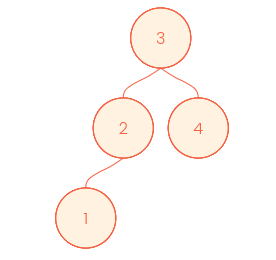
\includegraphics[scale=0.6]{true_optima.png}
\end{figure}

O custo $P$ da árvore é:
\begin{equation}
    P = 3 \cdot 1 + 2 \cdot 2 + 4 \cdot 2 + 1 \cdot 3 = 18
    \notag
\end{equation}

E nessa árvore ótima podemos observar que o elemento com o maior número de
acesso $p_{i}$ não está na raíz da árvore, e sim no segundo nível, confirmando
que uma solução gulosa para o algoritmo não funciona.


\problem{16} Problema 15-7 do CLRS (Programando para maximizar o lucro) Suponha
que você tem uma máquina e um conjunto de n trabalhos, identificados pelos
números $1, 2, . . . , n$, para processar nessa máquina. Cada trabalho $j$ tem
um tempo de processamento $t_{j}$ , um lucro $p{j}$ e um prazo final dj . A
máquina só pode processar um trabalho de cada vez, e o trabalho $j$ deve ser
executado ininterruptamente por tj unidades de tempo consecutivas. Se o trabalho
$j$ for concluído em seu prazo $d_{j}$ , você recebe um lucro $p_{j}$ , mas, se
ele for completado depois do seu prazo final, você não recebe nenhum lucro.
Escreva um algoritmo para encontrar a ordem de execução dos trabalho que
maximiza a soma dos lucros, supondo que todos os tempos de processamento são
inteiros entre $1$ e $n$. Qual é o tempo de execução do seu algoritmo?

\end{document}